%! TEX program = xelatex

\documentclass{article}
\usepackage[a4paper, margin=3cm]{geometry}
\setlength{\parindent}{0pt}
\setlength{\parskip}{1em}
\usepackage{graphicx}
\usepackage{fontspec}
\setmainfont{Lato}

\usepackage{amsmath,amssymb,amsthm}
%\usepackage{pgfplots}
%\pgfplotsset{compat=1.16}

\title{}
\author{Mikael Myyrä}
\date{}

\begin{document}

\section*{1.}

\[
  \begin{bmatrix}
    \,(2 + h^2) & -1 & & \,\\
    -1 & (2 + h^2) & -1 & \\
    \qquad \qquad \ddots & \qquad \ddots & \qquad \ddots \\
    & -1 & (2 + h^2) & -1 \\
    & & -1 & (2 + h^2) \\
  \end{bmatrix}
  \begin{bmatrix}
    \,u_1\, \\ u_2 \\ \vdots \\ u_{N-2} \\ u_{N-1}
  \end{bmatrix}
  =
  \begin{bmatrix}
    \,1\, \\ 0 \\ \vdots \\ 0 \\ 1
  \end{bmatrix}
\]
Merkitään funktion arvojen $u_k$ vektoria $\mathbf{u}$:lla.

Jakamalla puolittain $h^2$:lla ja erottamalla kerroinmatriisista
$h$:sta riippuvat termit saadaan
\[
  \frac{1}{h^2}
  \begin{bmatrix}
    \,2 & -1 & & \,\\
    -1 & 2 & -1 & \\
    & \ddots & \ddots & \ddots & \\
    & -1 & 2 & -1 \\
    & & -1 & 2 \\
  \end{bmatrix}
  \mathbf{u}
  +
  \mathbf{u}
  =
  \frac{1}{h^2}
  \begin{bmatrix}
    \,1\, \\ 0 \\ \vdots \\ 0 \\ 1
  \end{bmatrix}
\]
Tämä vastaa yhtälöryhmää
\[
  \begin{cases}
    \frac{1}{h^2}(2u_1 - u_2) + u_1 = \frac{1}{h^2} \\
    \frac{1}{h^2}(-u_1 + 2u_2 - u_3) + u_2 = 0 \\
    \vdots \\
    \frac{1}{h^2}(-u_{N-3} + 2u_{N-2} - u_{N-1}) + u_{N-2} = 0 \\
    \frac{1}{h^2}(-u_{N-2} + 2u_{N-1}) + u_{N-1} = \frac{1}{h^2} \\
  \end{cases}
\]
Reunimmaiset yhtälöt saadaan saman muotoisiksi kuin muut vähentämällä
oikeanpuoleiset termit:
\[
  \begin{cases}
    \frac{1}{h^2}(-1 + 2u_1 - u_2) + u_1 = 0 \\
    \frac{1}{h^2}(-u_1 + 2u_2 - u_3) + u_2 = 0 \\
    \vdots \\
    \frac{1}{h^2}(-u_{N-3} + 2u_{N-2} - u_{N-1}) + u_{N-2} = 0 \\
    \frac{1}{h^2}(-u_{N-2} + 2u_{N-1} - 1) + u_{N-1} = 0 \\
  \end{cases}
\]
Nyt tehtävä voidaan esittää pyydetyssä muodossa:
\begin{gather*}
  -\frac{u_{k-1} - 2u_k + u_{k+1}}{h^2} + u_k = 0, \quad k = 1,\dots,N-1 \\
  u_0 = 1, \\
  u_N = 1. \\
\end{gather*}

Tämä on differenssimenetelmällä diskretoitu muoto yhtälöstä
\[
  -\frac{\partial^2 u}{\partial x^2} + u = 0.
\]

\newpage

\section*{2.}

\subsection*{(a)}

\[
  -\frac{\partial^2 u}{\partial x^2} + \beta u(x) = f(x) \\
\]
Laskentavälillä $(0, 1)$, jonka pituus on 1 ja siis laskentapisteiden välimatka
on $\frac{1}{N}$.

\subsubsection*{i)}

Differenssimenetelmällä saadaan diskreetti tehtävä
\[
  \frac{1}{h^2}
  \begin{bmatrix}
    \,(2 + \beta h^2) & -1 && \,\\
     -1 & (2 + \beta h^2) & -1 & \\
      \qquad \quad \ddots &  \qquad \quad \ddots & \qquad \quad \ddots & \\
     & -1 & (2 + \beta h^2) & -1  \\
     & & -1 & (2 + \beta h^2) \\
  \end{bmatrix}
  \begin{bmatrix}
    u_1 \\ u_2 \\ \vdots \\ u_{N-2} \\ u_{N-1}
  \end{bmatrix}
  =
  \begin{bmatrix}
    f_1 + \frac{u_0}{h^2} \\ f_2 \\ \vdots \\ f_{N-2} \\ f_{N-1} + \frac{u_N}{h^2}
  \end{bmatrix}
\]
missä $f_k$ on funktion $f(x)$ arvo pisteessä $0 + kh$ = $\frac{k}{N}$.
Ratkaistaan matlabilla:

\begin{verbatim}
% parametrit
beta = 0;
u0 = 0;
uN = 0;
f = @(x) x - x^2;

function result = solveAndPlot(beta, u0, uN, f, stepCount)
  stepLength = 1 / stepCount;
  stepInvSq = 1 / stepLength^2;
  % u:n kerroinmatriisi
  uCoefs = zeros(stepCount - 1, stepCount - 1);
  uCoefs(1, 1) = 2 * stepInvSq + beta;
  for i = 2 : stepCount - 1
    uCoefs(i, i) = 2 * stepInvSq + beta;
    uCoefs(i, i-1) = -1 * stepInvSq;
    uCoefs(i-1, i) = -1 * stepInvSq;
  end

  % yhtalon oikea puoli
  rhs = zeros(stepCount - 1, 1);
  % ei paatepisteita mukaan
  x = stepLength : stepLength : 1 - stepLength;
  for i = 1 : stepCount - 1
    rhs(i) = f(x(i));
  end
  rhs(1) = rhs(1) + u0 * stepInvSq;
  rhs(stepCount - 1) = rhs(stepCount - 1) + uN * stepInvSq;

  result = uCoefs \ rhs;
  result = [u0; result; uN];

  plot(0:stepLength:1, result, '-o')
  xlabel('x')
  ylabel('u')
  hold on
end

stepCounts = [10 20 40];
for i = 1 : length(stepCounts)
  solveAndPlot(beta, u0, uN, f, stepCounts(i));
end
\end{verbatim}

\begin{center}
\includegraphics[width=350pt]{html/w3_2ai-1.jpg}
\end{center}

Näyttää siltä, että hilaväli ei juurikaan vaikuta ratkaisuun.
Käyriä on vaikea erottaa toisistaan. Huomattava ero on vain paraabelin
huipulla, missä käyrän kaarevuus on suurimmillaan.

\subsubsection*{ii)}

Neumann-reunaehdon kanssa myös välin päätepisteet tarvitaan mukaan ratkaistavaan vektoriin.
Approksimoidaan reunaehtoja yksipuolisilla differensseillä $\frac{u_1 - u_0}{h} = du_0 = 0$
ja $\frac{u_N - u_{N-1}}{h} = du_N = e - \frac{1}{e}$. Nämä saadaan mukaan matriisitehtävään
kasvattamalla matriiseja seuraavasti:
\[
  \frac{1}{h^2}
  \begin{bmatrix}
    \,1 & -1 \\
    -1 & (2 + \beta h^2) & -1 \\
       & -1 & (2 + \beta h^2) & -1 \\
       & \qquad \quad \ddots &  \qquad \quad \ddots & \qquad \quad \ddots \\
    & & -1 & (2 + \beta h^2) & -1  \\
    & & & -1 & (2 + \beta h^2) & -1 \\
    & & & & -1 & 1 \, \\
  \end{bmatrix}
  \begin{bmatrix}
    u_0 \\ u_1 \\ u_2 \\ \vdots \\ u_{N-2} \\ u_{N-1} \\ u_N
  \end{bmatrix}
  =
  \begin{bmatrix}
    -\frac{du_0}{h} \\ f_1 \\ f_2 \\ \vdots \\ f_{N-2} \\ f_{N-1} \\ \frac{du_N}{h}
  \end{bmatrix}
\]

Matlab-koodi on melkein sama kuin edellisessä:

\begin{verbatim}
% parametrit
beta = 1;
du0 = 0;
duN = exp(1) - 1/exp(1);
f = @(x) 0;

function result = solveAndPlot(beta, du0, duN, f, stepCount)
  stepLength = 1 / stepCount;
  stepInvSq = 1 / stepLength^2;
  % u:n kerroinmatriisi
  uCoefs = zeros(stepCount + 1, stepCount + 1);
  uCoefs(1, 1) = stepInvSq;
  for i = 2 : stepCount + 1
    uCoefs(i, i) = 2 * stepInvSq + beta;
    uCoefs(i, i-1) = -1 * stepInvSq;
    uCoefs(i-1, i) = -1 * stepInvSq;
  end
  uCoefs(stepCount + 1, stepCount + 1) = stepInvSq;

  % yhtalon oikea puoli
  rhs = zeros(stepCount + 1, 1);
  x = 0 : stepLength : 1;
  for i = 1 : stepCount
    rhs(i) = f(x(i));
  end
  rhs(1) = du0 / stepLength;
  rhs(stepCount + 1) = duN / stepLength;

  result = uCoefs \ rhs;

  plot(x, result, '-o')
  xlabel('x')
  ylabel('u')
  hold on
end

stepCounts = [10 20 40 80];
for i = 1 : length(stepCounts)
  solveAndPlot(beta, du0, duN, f, stepCounts(i));
end
\end{verbatim}

\begin{center}
\includegraphics[width=350pt]{html/w3_2aii-1.jpg}
\end{center}

Tässä hilavälillä on suurempi vaikutus. Mitä suurempi väli, sitä korkeammalle
koko käyrä asettuu. Dirichlet-reunaehtojen kanssa tätä ei voinut tapahtua,
koska ne eivät salli reunapisteiden liikkumista.

\subsection*{(b)}

i)-tehtävän tunnettu ratkaisu on $u(x) = \frac{1}{12}(x^4 - 2x^3 + x)$.
Wolfram Alpha antaa tehtävän ii) ratkaisuksi $u(x) = e^{-x} + e^x$. Lisäsin
molempien tehtävien matlab-koodiin seuraavanlaisen pätkän, joka tulostaa
tunnetun ratkaisun ja diskreetin tehtävän ratkaisun erotuksen euklidisen
normin:

\begin{verbatim}
stepCounts = [10 20 40 80];
knownSolution = @(x) exp(-x) + exp(x);
for i = 1 : length(stepCounts)
  result = solveAndPlot(beta, du0, duN, f, stepCounts(i));

  x = 0 : 1 / stepCounts(i) : 1;
  accurateResult = zeros(stepCounts(i) + 1, 1);
  for i = 1 : stepCounts(i) + 1
    accurateResult(i) = knownSolution(x(i));
  end

  diff = result - accurateResult;
  diffNorm = norm(diff)
end
\end{verbatim}

Sain seuraavat tulokset:

\begin{center}
  \begin{tabular}{|c|c|c|c|c|}
    \hline
    h & $\frac{1}{10}$ & $\frac{1}{20}$ & $\frac{1}{40}$ & $\frac{1}{80}$ \\
    \hline\hline
    i) & 0.00048110 & 0.00017010 & 0.000060141 & 0.000021263 \\
    \hline
    ii) & 0.94638 & 0.61672 & 0.41890 & 0.29035 \\
    \hline
  \end{tabular}
\end{center}

\newpage

\section*{3.}

\[
  -\frac{\partial^2 u}{\partial x^2} - \frac{\partial^2 u}{\partial y^2} = \sin(x)\sin(2y)
\]
Tässä toimii luennoilta tuttu diskretointi
\[
  \frac{-u_{i,j-1} - u_{i-1,j} + 4u_{i,j} - u_{i+1,j} - u_{i,j+1}}{h^2} = f_{i,j}.
\]
Matlab-koodi:
\begin{verbatim}
f = @(x,y) sin(x)*sin(2*y);
leftEdge = @(y) 0;
rightEdge = @(y) 0;
bottomEdge = @(x) 0;
topEdge = @(x) sin(x);

STEP_COUNT = 4;
INNER_STEP_COUNT = STEP_COUNT - 1;
STEP_LENGTH = pi / STEP_COUNT;
STEP_LENGTH_SQ = STEP_LENGTH^2;

% u:n kerroinmatriisi lohkomatriisina
blockT = diag(4*ones(INNER_STEP_COUNT, 1)) ...
       - diag(ones(INNER_STEP_COUNT - 1, 1), 1) ...
       - diag(ones(INNER_STEP_COUNT - 1, 1), -1);
sideDiag = -ones(INNER_STEP_COUNT^2 - 3, 1);
uCoefs = blkdiag(repmat({blockT}, 1, INNER_STEP_COUNT){:}) ...
       + diag(sideDiag, 3) ...
       + diag(sideDiag, -3);

% yhtalon oikea puoli
rhs = zeros(INNER_STEP_COUNT^2, 1);
% ei reunoja mukaan
x = STEP_LENGTH : STEP_LENGTH : pi - STEP_LENGTH;
y = STEP_LENGTH : STEP_LENGTH : pi - STEP_LENGTH;
for xi = 1 : INNER_STEP_COUNT
  for yi = 1 : INNER_STEP_COUNT
    rhsIdx = (yi-1) * INNER_STEP_COUNT + xi;
    rhs(rhsIdx) = STEP_LENGTH_SQ * f(x(xi), y(yi));
    % reuna-arvot
    if xi == 1
      rhs(rhsIdx) = rhs(rhsIdx) + leftEdge(y(yi));
    elseif xi == INNER_STEP_COUNT
      rhs(rhsIdx) = rhs(rhsIdx) + rightEdge(y(yi));
    end
    if yi == 1
      rhs(rhsIdx) = rhs(rhsIdx) + bottomEdge(x(xi));
    elseif yi == INNER_STEP_COUNT
      rhs(rhsIdx) = rhs(rhsIdx) + topEdge(x(xi));
    end
  end
end

solution = uCoefs \ rhs;

% piirto
% tarvitaan ratkaisu 2D-matriisina, lisataan myos mukaan reuna-arvot
solM = zeros(STEP_COUNT + 1, STEP_COUNT + 1);
for xi = 1 : INNER_STEP_COUNT
  for yi = 1 : INNER_STEP_COUNT
    solM(xi+1, yi+1) = solution((yi-1) * INNER_STEP_COUNT + xi);
  end
end
% reuna-arvot
x = 0 : STEP_LENGTH : pi;
y = 0 : STEP_LENGTH : pi;
solM(1, :) = leftEdge(y);
solM(STEP_COUNT + 1, :) = rightEdge(y);
solM(:, 1) = bottomEdge(x);
solM(:, STEP_COUNT + 1) = topEdge(x);

surf(x, y, solM)
xlabel('x')
ylabel('y')
zlabel('u')

\end{verbatim}

Lopputulos hilavälillä $\frac{\pi}{4}$:

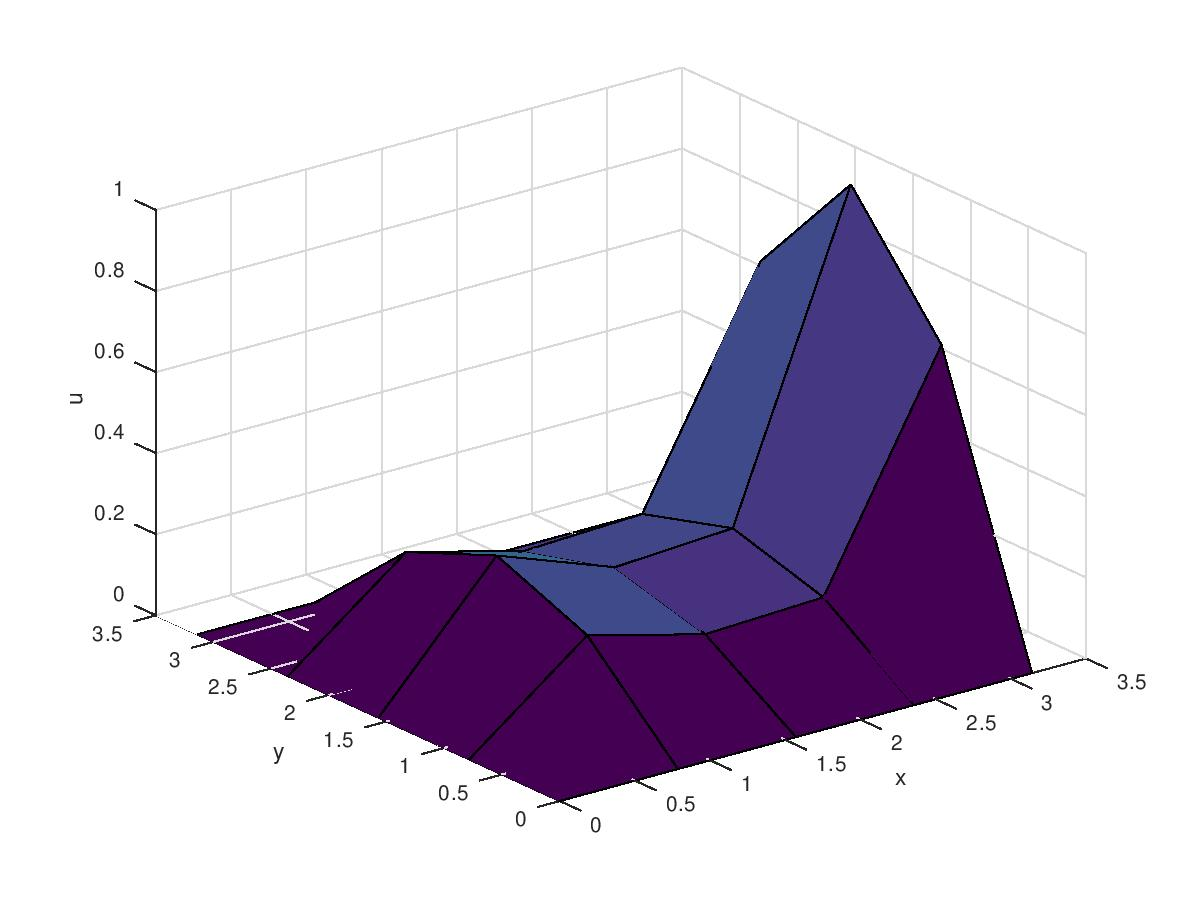
\includegraphics[width=350pt]{w3_3-4p.jpg}

ja hilavälillä $\frac{\pi}{10}$:

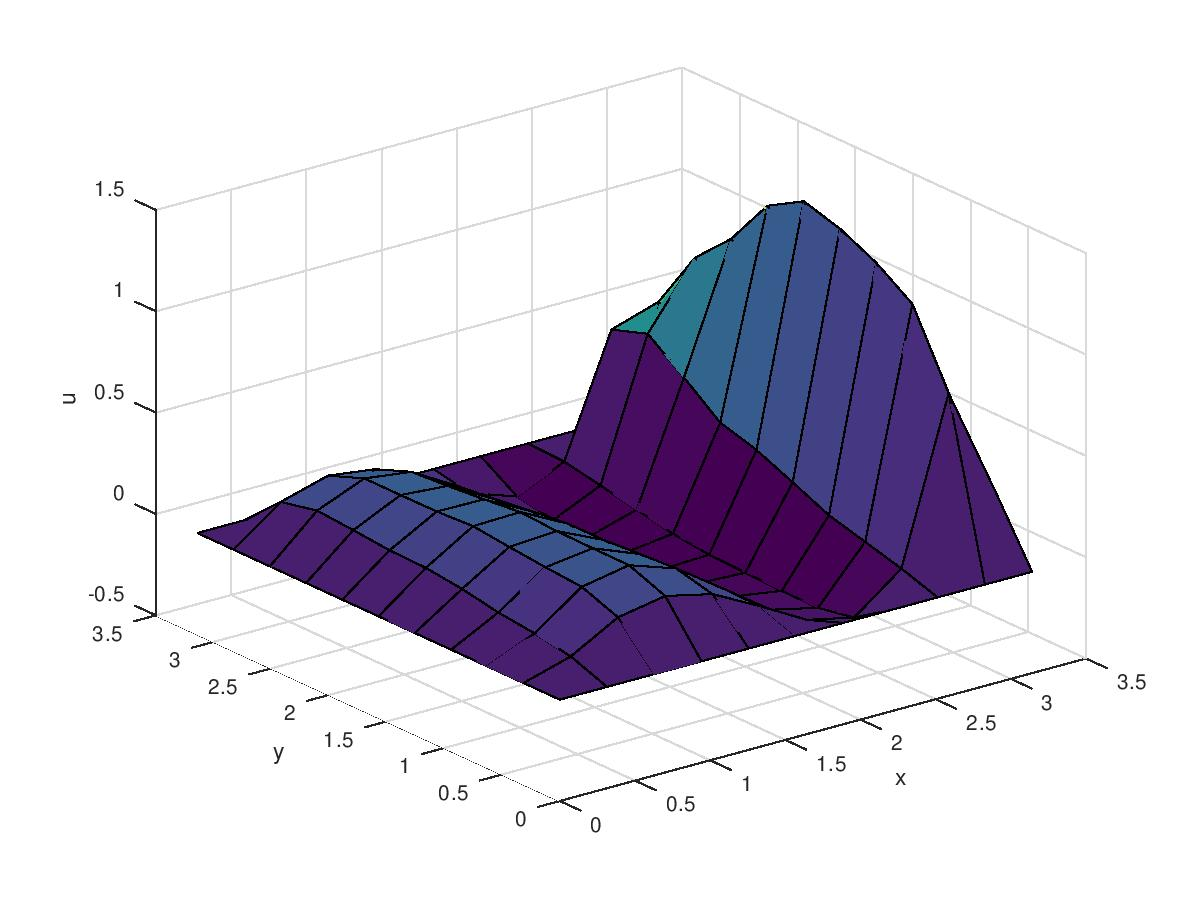
\includegraphics[width=350pt]{w3_3-10p.jpg}

\end{document}
